\section{Resultados y Análisis}

%%%%%%%%%%%%%%%%%%%%%%%%%%%%%%%%%%%%%%%%%%%%%%%%%%%%%%%%%%%%%%%%%%%%%%%%%
%%%%%%%%%%%%%%%%%%%%%%%%%%%%%%%%%%%%%%%%%%%%%%%%%%%%%%%%%%%%%%%%%%%%%%%%%

\subsection{Resultados}

%%%%%%%%%%%%%%%%%%%%%%%%%%%%%%%%%%%%%%%%%%%%%%%%%%%%%%%%%%%%%%%%%%%%%%%%%

\begin{frame}{Resultados del conjunto de modelos estudiados}

    \begin{columns}
        
    \column{0.5\textwidth}\centering
    \begin{table}[H]
        \begin{center}
        \resizebox{0.95\columnwidth}{!}{
        \begin{tabular}{|l|r|r|r|r|r|}
        \hline
        \textbf{} & \multicolumn{1}{l|}{\textbf{Fn}} & \multicolumn{1}{l|}{\textbf{Fa}} & \multicolumn{1}{l|}{\textbf{Fo}} & \multicolumn{1}{l|}{\textbf{Fr}} & \multicolumn{1}{l|}{\textbf{F1}} \\ \hline
        \textbf{B. Cascada} & 0,916 & 0,827 & 0,786 & 0,617 & 0,787 \\ \hline
        \textbf{R.F.} & 0,892 & 0,768 & 0,722 & 0,584 & 0,741 \\ \hline
        \textbf{CNN} & 0,879 & 0,736 & 0,634 & 0,519 & 0,692 \\ \hline
        \textbf{GRU} & 0,871 & 0,668 & 0,592 & 0,442 & 0,643 \\ \hline
        \textbf{LSTM} & 0,849 & 0,312 & 0,525 & 0,361 & 0,511 \\ \hline
        \textbf{OhShuLi} & 0,793 & 0,193 & 0,31 & 0,249 & 0,386 \\ \hline
        \textbf{ChenChen} & 0,776 & 0,149 & 0,192 & 0,088 & 0,301 \\ \hline
        \textbf{GaoJunLi} & 0,743 & 0 & 0,034 & 0,068 & 0,211 \\ \hline
        \end{tabular}}
        \end{center}
        \label{table:Comparativa Global}
    \end{table}
    
    
    \column{0.5\textwidth}\centering
    \begin{figure}
        \centering
        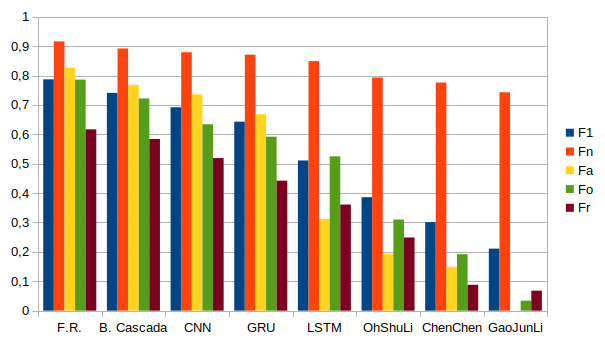
\includegraphics[width=\linewidth]{Images/grafica comparativa.png}
    \end{figure}
    \end{columns}
    
    \pause

    Ranking:
    \pause

    \begin{enumerate}
        \item Modelos de la competición
        \item Modelos propios
        \item Propuestas de la literatura
    \end{enumerate}
    
    
\end{frame}

%%%%%%%%%%%%%%%%%%%%%%%%%%%%%%%%%%%%%%%%%%%%%%%%%%%%%%%%%%%%%%%%%%%%%%%%%

\subsection{Análisis}

\begin{frame}{Modelos de la competición}
\begin{columns}
    \column{0.5\textwidth}\centering
        \begin{table}[H]
        \vspace{-1cm}
        \caption{Clasf. RF}
        \begin{center}
        \resizebox{\columnwidth}{!}{%
        \begin{tabular}{|c|r|r|r|r|}
        \hline
        \multicolumn{1}{|l|}{} & \multicolumn{1}{l|}{\textbf{Normal}} & \multicolumn{1}{l|}{\textbf{FA}} & \multicolumn{1}{l|}{\textbf{Otro}} & \multicolumn{1}{l|}{\textbf{Ruido}} \\ \hline
        \textbf{Normal} & 953 & 2 & 57 & 3 \\ \hline
        \textbf{FA} & 5 & 116 & 29 & 2 \\ \hline
        \textbf{Otro} & 92 & 10 & 375 & 6 \\ \hline
        \textbf{Ruido} & 15 & 1 & 10 & 29 \\ \hline
        \end{tabular}}
        \end{center}
        \end{table}
        
        
        \begin{table}[H]
        %\vspace{-1cm}
        \caption{Clasf. Binario en Cascada}
        \begin{center}
        \resizebox{\columnwidth}{!}{%
        \begin{tabular}{|c|r|r|r|r|}
        \hline
        \multicolumn{1}{|l|}{} & \multicolumn{1}{l|}{\textbf{Normal}} & \multicolumn{1}{l|}{\textbf{FA}} & \multicolumn{1}{l|}{\textbf{Otro}} & \multicolumn{1}{l|}{\textbf{Ruido}} \\ \hline
        \textbf{Normal} & 962 & 7 & 53 & 6 \\ \hline
        \textbf{FA} & 6 & 114 & 28 & 4 \\ \hline
        \textbf{Otro} & 118 & 21 & 333 & 10 \\ \hline
        \textbf{Ruido} & 15 & 4 & 7 & 31 \\ \hline
        \end{tabular}}
        \end{center}
        \end{table}
    
    
    \column{0.5\textwidth}\centering
    \begin{itemize}
        \item Mejores resultados, aunque lejos de la perfección
        \item Dificultad para distinguir Ritmo normal frente a otras patologías distintas de FA
        \item Conocimiento a priori.
        \item Modelos específicos diseñados para el problema
    \end{itemize}
\end{columns}       
\end{frame}

%%%%%%%%%%%%%%%%%%%%%%%%%%%%%%%%%%%%%%%%%%%%%%%%%%%%%%%%%%%%%%%%%%%%%%%%%

\begin{frame}{Modelos de la literatura}
\begin{columns}
    \column{0.5\textwidth}\centering
        \begin{table}[H]
        \caption{GaoJunLi}
        \begin{center}
        \resizebox{\columnwidth}{!}{%
        \begin{tabular}{|l|r|r|r|r|}
        \hline
         & \multicolumn{1}{l|}{\textbf{Normal}} & \multicolumn{1}{l|}{\textbf{FA}} & \multicolumn{1}{l|}{\textbf{Otro}} & \multicolumn{1}{l|}{\textbf{Ruido}} \\ \hline
        \textbf{Normal} & 1111 & 0 & 0 & 0 \\ \hline
        \textbf{FA} & 147 & 0 & 0 & 0 \\ \hline
        \textbf{Otro} & 491 & 0 & 0 & 0 \\ \hline
        \textbf{Ruido} & 36 & 0 & 0 & 0 \\ \hline
        \end{tabular}}
        \end{center}
        \end{table}
        
        \begin{table}[H]
        %\vspace{-1cm}
        \caption{ChenChen}
        \begin{center}
        \resizebox{\columnwidth}{!}{%
        \begin{tabular}{|l|r|r|r|r|}
        \hline
         & \multicolumn{1}{l|}{\textbf{Normal}} & \multicolumn{1}{l|}{\textbf{FA}} & \multicolumn{1}{l|}{\textbf{Otro}} & \multicolumn{1}{l|}{\textbf{Ruido}} \\ \hline
        \textbf{Normal} & 973 & 2 & 92 & 0 \\ \hline
        \textbf{FA} & 122 & 1 & 11 & 0 \\ \hline
        \textbf{Otro} & 431 & 2 & 43 & 0 \\ \hline
        \textbf{Ruido} & 35 & 0 & 1 & 0 \\ \hline
        \end{tabular}}
        \end{center}
        \end{table}
    
    
    \column{0.5\textwidth}\centering
    
        \begin{table}[H]
        \vspace{-1cm}
        \caption{OhShuLi}
        \begin{center}
        \resizebox{\columnwidth}{!}{%
        \begin{tabular}{|l|r|r|r|r|}
        \hline
         & \multicolumn{1}{l|}{\textbf{Normal}} & \multicolumn{1}{l|}{\textbf{FA}} & \multicolumn{1}{l|}{\textbf{Other}} & \multicolumn{1}{l|}{\textbf{Ruido}} \\ \hline
        \textbf{Normal} & 980 & 0 & 29 & 0 \\ \hline
        \textbf{FA} & 141 & 0 & 6 & 0 \\ \hline
        \textbf{Other} & 470 & 0 & 20 & 0 \\ \hline
        \textbf{Ruido} & 30 & 0 & 5 & 0 \\ \hline
        \end{tabular}}
        \end{center}
        \end{table}
        
    \begin{itemize}
        \item No son capaces de clasificar adecuadamente
        \item Modelos diseñados para otro problema
        \item Peores Resultados
    \end{itemize}
\end{columns}       
\end{frame}

%%%%%%%%%%%%%%%%%%%%%%%%%%%%%%%%%%%%%%%%%%%%%%%%%%%%%%%%%%%%%%%%%%%%%%%%%

\begin{frame}{Modelos propios}
\begin{columns}
    \column{0.5\textwidth}\centering
        \begin{table}[H]
        \caption{CNN}
        \begin{center}
        \resizebox{\columnwidth}{!}{%
        \begin{tabular}{|l|r|r|r|r|}
        \hline
         & \multicolumn{1}{l|}{\textbf{Normal}} & \multicolumn{1}{l|}{\textbf{FA}} & \multicolumn{1}{l|}{\textbf{Otras}} & \multicolumn{1}{l|}{\textbf{Ruido}} \\ \hline
        \textbf{Normal} & 941 & 6 & 62 & 0 \\ \hline
        \textbf{FA} & 117 & 10 & 20 & 0 \\ \hline
        \textbf{Otras} & 371 & 9 & 110 & 0 \\ \hline
        \textbf{Ruido} & 29 & 1 & 6 & 0 \\ \hline
        \end{tabular}}
        \end{center}
        \end{table}
        
        \begin{table}[H]
        %\vspace{-1cm}
        \caption{LSTM}
        \begin{center}
        \resizebox{\columnwidth}{!}{%
        \begin{tabular}{|l|r|r|r|r|}
        \hline
        \textbf{} & \multicolumn{1}{l|}{\textbf{Normal}} & \multicolumn{1}{l|}{\textbf{FA}} & \multicolumn{1}{l|}{\textbf{Otras}} & \multicolumn{1}{l|}{\textbf{Ruido}} \\ \hline
        \textbf{Normal} & 927 & 0 & 82 & 0 \\ \hline
        \textbf{FA} & 127 & 0 & 20 & 0 \\ \hline
        \textbf{Otras} & 422 & 0 & 68 & 0 \\ \hline
        \textbf{Ruido} & 30 & 0 & 6 & 0 \\ \hline
        \end{tabular}}
        \end{center}
        \end{table}
    
    
    \column{0.5\textwidth}\centering
    
        \begin{table}[H]
        \vspace{-1cm}
        \caption{GRU}
        \begin{center}
        \resizebox{\columnwidth}{!}{%
        \begin{tabular}{|l|r|r|r|r|}
        \hline
        \textbf{} & \multicolumn{1}{l|}{\textbf{Normal}} & \multicolumn{1}{l|}{\textbf{FA}} & \multicolumn{1}{l|}{\textbf{Otras}} & \multicolumn{1}{l|}{\textbf{Ruido}} \\ \hline
        \textbf{Normal} & 934 & 6 & 69 & 0 \\ \hline
        \textbf{FA} & 114 & 6 & 27 & 0 \\ \hline
        \textbf{Otras} & 375 & 9 & 106 & 0 \\ \hline
        \textbf{Ruido} & 29 & 1 & 6 & 0 \\ \hline
        \end{tabular}}
        \end{center}
        \end{table}
        
    \begin{itemize}
        \item No son capaces de clasificar la clase minoritaria
        \item Problemas en distinguir Normal frente a Otro y FA
    \end{itemize}
\end{columns}       
\end{frame}

%%%%%%%%%%%%%%%%%%%%%%%%%%%%%%%%%%%%%%%%%%%%%%%%%%%%%%%%%%%%%%%%%%%%%%%%%
%%%%%%%%%%%%%%%%%%%%%%%%%%%%%%%%%%%%%%%%%%%%%%%%%%%%%%%%%%%%%%%%%%%%%%%%%


